\documentclass{article}[12pt]

% useful packages
\usepackage{fullpage}
\usepackage{amsmath,amssymb,amsthm,amsfonts}
\usepackage{graphicx}
\usepackage{enumerate}
\usepackage{algorithm,algorithmic}
\usepackage{xcolor}
\usepackage{bbm}
\usepackage{url}
\usepackage{caption,subcaption}

% theorem type environments
\newtheorem{thm}{Theorem}
\newtheorem{prop}{Proposition}
\newtheorem{lemma}{Lemma}
\newtheorem{cor}{Corollary}
\newtheorem{defn}{Definition}
\newtheorem{assump}{Assumption}
\newtheorem{example}{Example}
\newtheorem{conjecture}{Conjecture}

% frequently used symbols
\newcommand{\bE}{\mathbb{E}}
\newcommand{\bP}{\mathbb{P}}
\newcommand{\bQ}{\mathbb{Q}}
\newcommand{\bR}{\mathbb{R}}
\newcommand{\bS}{\mathbb{S}}
\newcommand{\bN}{\mathbb{N}}
\newcommand{\bZ}{\mathbb{Z}}
\newcommand{\sC}{{\mathcal C}} 
\newcommand{\sD}{{\mathcal D}} 
\newcommand{\sE}{{\mathcal E}} 
\newcommand{\sF}{{\mathcal F}} 
\newcommand{\sL}{{\mathcal L}} 
\newcommand{\sH}{{\mathcal H}} 
\newcommand{\sN}{{\mathcal N}} 
\newcommand{\sO}{{\mathcal O}} 
\newcommand{\sP}{{\mathcal P}} 
\newcommand{\sR}{{\mathcal R}} 
\newcommand{\sS}{{\mathcal S}}
\newcommand{\sU}{{\mathcal U}} 
\newcommand{\sX}{{\mathcal X}} 
\newcommand{\sY}{{\mathcal Y}} 
\newcommand{\sZ}{{\mathcal Z}}

% operators
\newcommand{\sign}{\mathop{\mathrm{sign}}}
\newcommand{\supp}{\mathop{\mathrm{supp}}} % support
\newcommand{\argmin}{\operatornamewithlimits{arg\ min}}
\newcommand{\argmax}{\operatornamewithlimits{arg\ max}}
\newcommand{\dist}{\operatorname{dist}}
\newcommand{\tr}{\text{tr}}
\newcommand{\vecop}{\text{vec}}
\newcommand{\st}{\operatorname{s.t.}}
\newcommand{\cut}{\setminus}
\newcommand{\ra}{\rightarrow}
\newcommand{\ind}[1]{\mathbbm{1}\left\{#1\right\}} 
\newcommand{\given}{\ | \ }

% grouping operators
\newcommand{\brac}[1]{\left[#1\right]}
\newcommand{\set}[1]{\left\{#1\right\}}
\newcommand{\abs}[1]{\left\lvert #1 \right\rvert}
\newcommand{\paren}[1]{\left(#1\right)}
\newcommand{\norm}[1]{\left\|#1\right\|}
\newcommand{\ip}[2]{\left\langle #1,#2 \right\rangle}

% code commands
\newcommand{\matlab}{\textsc{Matlab }}
\newcommand{\algname}[1]{\textnormal{\textsc{#1}}}

% header command
\newcommand{\homework}[4]{
    \pagestyle{myheadings}
    \thispagestyle{plain}
    \newpage
    \setcounter{page}{1}
    \setlength{\headsep}{10mm}
    \noindent
    \begin{center}
    \framebox{
        \vbox{\vspace{2mm}
            \hbox to 6.28in { {\bf STAT 671: Statistical Learning I
            \hfill Fall 2019} }
        \vspace{4mm}
        \hbox to 6.28in { {\Large \hfill Homework #1 \hfill} }
        \vspace{2mm}
        \hbox to 6.28in { \Large \hfill Due: #2 \hfill }
        \vspace{2mm}
        \hbox to 6.28in { {\it Student Name: #3} \hfill {\it Professor Name: #4}}
        \vspace{2mm}}
   }
   \end{center}
   \markboth{Homework #1}{Homework #1}
   \vspace*{4mm}
}

\begin{document}

\homework{3}{November 6, 2019}{Ethan Lew}{Dr. Bruno Jedynak}

\section{Kernalized ridge regression}
\begin{enumerate}
\item Code the kernalized ridge regression for the 2d data that you already used for the simple classifier and the perceptron. Show your code. Note that an example code for 1d data is available in the folder \lq\lq{}code\rq\rq{} in d2l.   Show 3 examples of results obtain with simulated data in 2 dimensions, using 3 different kernels. 

\begin{figure}[H]
\centering
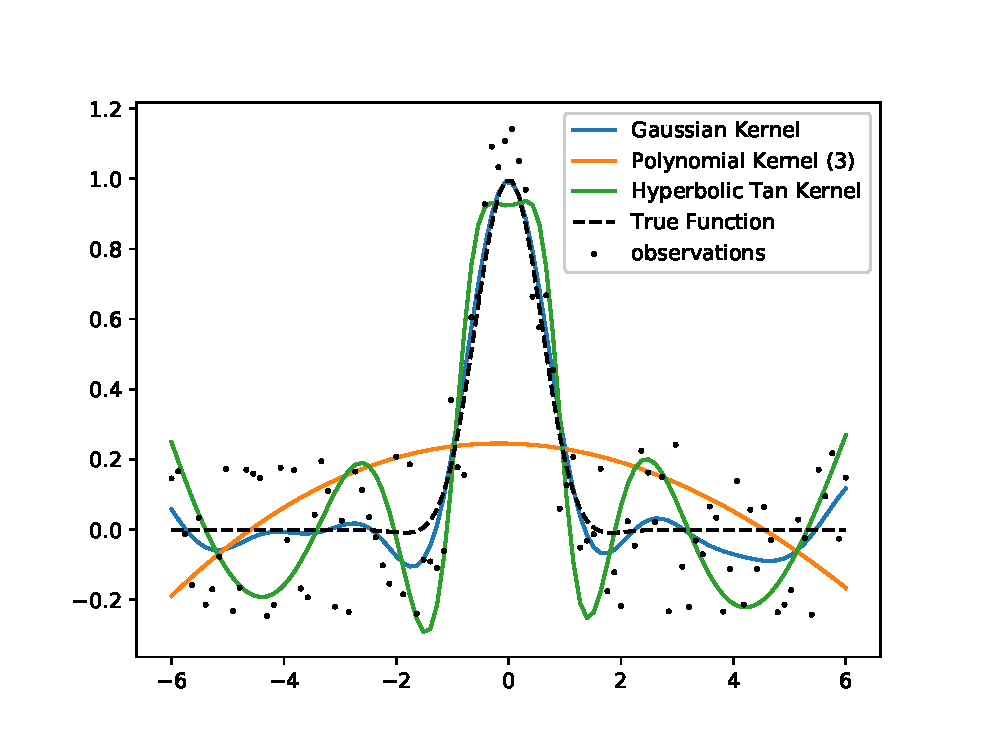
\includegraphics[width=0.7\textwidth]{./img/krr_k.eps}
\caption{Kernalized Ridge Regression  for 3 Kernels (1D)}
\end{figure}

\begin{figure}[H]
\centering
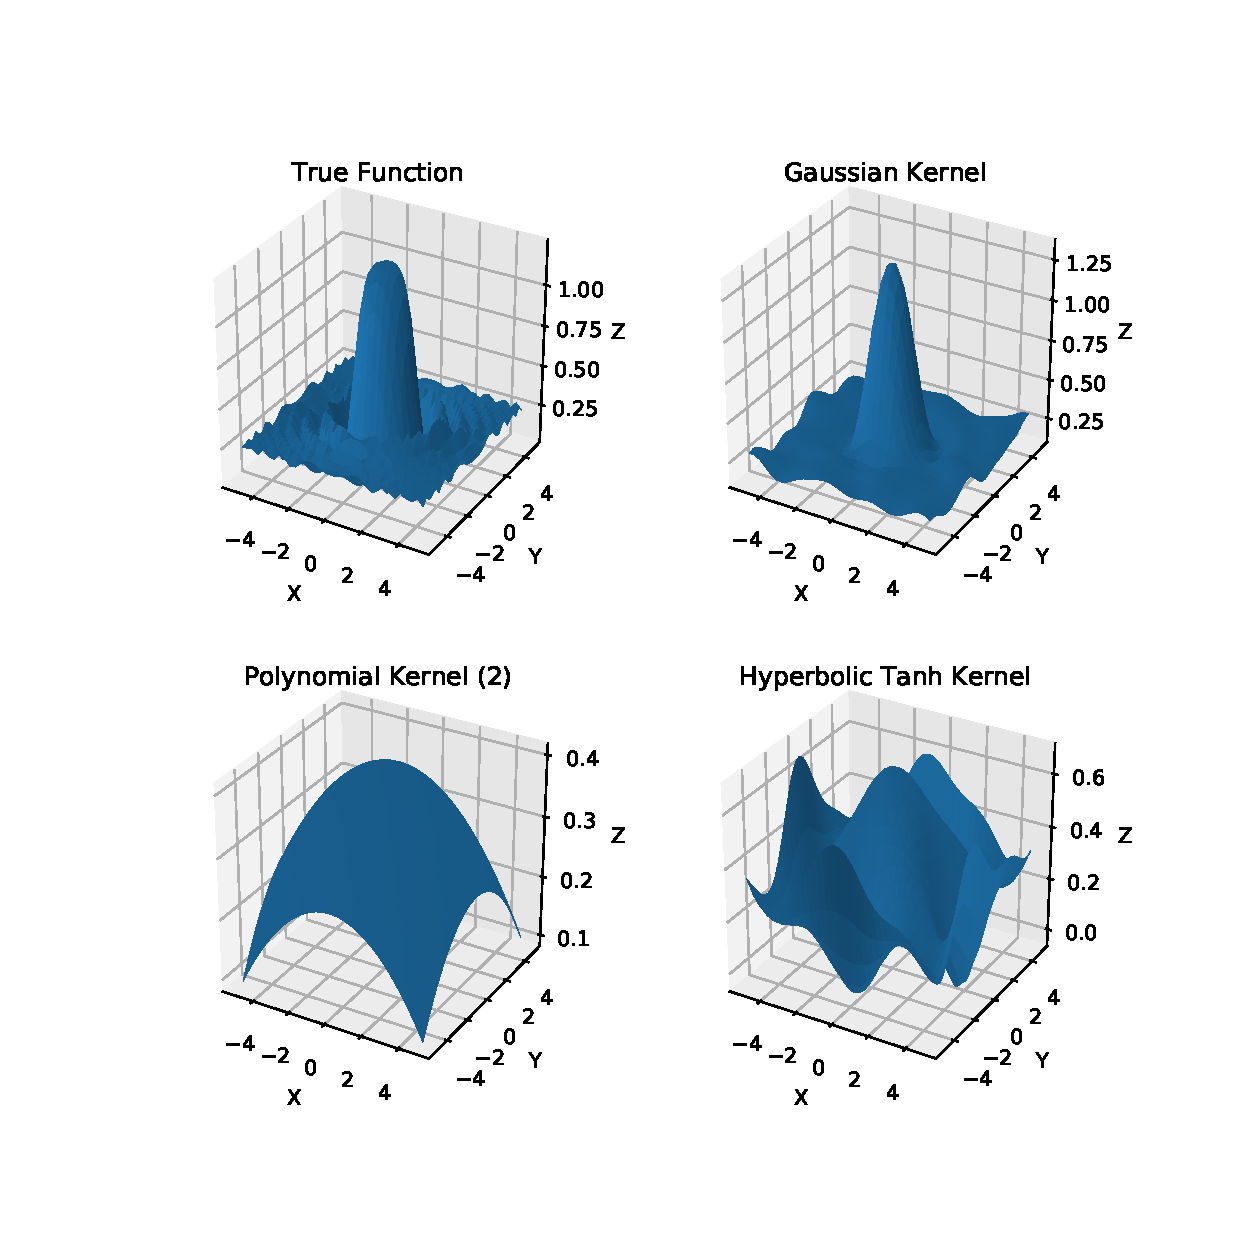
\includegraphics[width=0.9\textwidth]{./img/krr_k2.eps}
\caption{Kernalized Ridge Regression  for 3 Kernels (2D)}
\end{figure}


\item Import the MNIST dataset. It is available on D2L. A R file is available for reading the files and run a simple classifier.  You will find online similar code in case you use Python,  Matlab or other high level language. 

Code a version of the kernalized ridge regression algorithm that let you run the algorithm for various sets of images from the MNIST dataset such that you can perform controled experiments. The input of the algorithm could be a list of filenames, corresponding to images for training, testing, as well as the corresponding labels.  

Run the kernelized ridge regression for one digit versus another one of your choice. You will see that the size of the full MNIST training set might be too large for the algorithm to run in a reasonable time. Instead, sample smaller training sets, say of size 100. Now, you should be able to run the algorithm. Experiment with smaller and larger training set size. Report the performance by specifying the total number of images correctly classified, as well as the learning time and testing time. Show graphs, with on the horizontal axis the number of images used for training or for testing. 

\begin{figure}[H]
\centering
\includegraphics[width=0.7\textwidth]{./img/mnist_perf.eps}
\caption{MNIST Kernalized Ridge Regression Performance}
\end{figure}

\begin{table}[h]
\centering
\begin{tabular}{|c|c|c|c|c|} \hline
\multicolumn{5}{|c|}{Classification Between 0 and 1 Benchmark --- Intel Core i7-4790K} \\ \hline
 Training Size & Testing Size & Learning Time (s) & Testing Time (s) & Classification Error (\%) \\ \hline \hline
  148 & 1330 & 0.062 & 0.934 & 1.01 \\ \hline
  443 & 1035 & 0.505 & 1.807 & 0.531 \\ \hline
  739 & 739 & 1.225 & 2.318 & 0.203 \\ \hline
  1035 & 443 & 2.315 & 1.889 & 0.113 \\ \hline
  1330 & 148 & 3.817 & 0.849 & 0.003 \\ \hline
\end{tabular}

\end{table}

\begin{table}[h]
\centering
\begin{tabular}{|c||c|c|c|c|c|c|c|c|c|} \hline
\multicolumn{10}{|c|}{Classification Error Between Digits for $m=228$ ($\%$)} \\ \hline
Digit Pair &0& 1& 2& 3& 4& 5& 6& 7& 8 \\ \hline \hline
1 &0.45  & & & & & & & & \\ \hline
2 &3.11  &2.02  & & & & & & &\\ \hline
3 &3.55  &2.44  &2.59  & & & &  & &\\ \hline
4 &1.21  &2.04  &4.35  &1.67  & & & &  &\\ \hline
5 &4.04  &3.05  &3.77  &5.20  &3.55  & &  & &\\ \hline
6 &3.38  &3.62  &1.20  &1.90  &1.95  &3.54  & & &\\ \hline
7 &2.11  &1.76  &3.74  &2.30  &4.25  &2.45  &3.29  &  &\\ \hline
8 &2.18  &2.71  &3.86  &2.39  &4.15  &3.30  &3.66  &2.83   &\\ \hline
9 &2.88  &1.79  &2.39  &3.32  &5.31  &3.52  &1.21  &5.37  &3.14  \\ \hline
\end{tabular}
\end{table}
\end{enumerate}
%\section{Kernalized ridge regression}
%\begin{enumerate}
%\item Code the kernalized ridge regression for the 2d example that you already used for the simple classifier and the perceptron. Show your code.  
%\item Show 3 examples of results obtain with simulated data in 2 dimensions, using 3 different kernels. 
%\end{enumerate}
%\section{MNIST dataset}
%\begin{enumerate}
%\item Import the MNIST dataset. It is available on D2L. A R file is available for reading the files and run a simple classifier.  you will find online similar code in case you use Matlab or other high level language. 
%\item Try to run the kernelized ridge regression for the digit zero versus all the other ones.  You will see that the size of the training set is too large. Sample a smaller training set, say of size 100. Now, you should be able to run it. Experiment with larger training set size. Report the performances, learning time and testing time on a graph.   
%\end{enumerate}
\section{Semi-parametric regression}
Let $\mathcal{D}=\{(x_i,y_i), 1 \leq i \leq n\}$ be a training set where $x_i \in \mathbb{R}^d$ is a feature vector, and $y_i \in \mathbb{R}$ is the target, or independent variable. 

We are interested in the following semi-parametric model for predicting $y$, 
\begin{equation}
f(x) = \theta^T x + g(x)
\end{equation}
where $\theta \in \mathbb{R}^d$ is a vector of parameters and $g: \mathbb{R}^d \mapsto \mathbb{R}$ belongs to a RKHS with kernel $k(.,.)$. 

This model is called semi-parametric because it is the sum of a parametric component, here the linear term $\theta^T x$ and a non-linear component, the function $g(.)$. 

Consider the functional 
\begin{equation}
J(\theta,g) = \sum_{i=1}^n \left(y_i - \theta^T x_i - g(x_i)\right)^2 + \lambda ||g||_H^2
\end{equation}
\begin{enumerate}
\item 
Show that for any $\theta$, a function $g \in H$ that minimizes $J(\theta,g)$ has the following form 
\begin{equation}
g(.)=\sum_{i=1}^n \alpha_i k(x_i,.)
\end{equation}
where $\alpha \in \mathbb{R}^n$ 
\item 
Show that 
\begin{equation}
J(\sum_{i=1}^n \alpha_i k(x_i,.),\theta)=||y - X\theta - K\alpha||^2 + \lambda \alpha^T K \alpha
\end{equation}
for some matrix $K$ and $X$ which you will specify together with their dimensions. 
\item Compute $\nabla_\alpha J$, the gradient of $J$ with respect to $\alpha$. Similarly, compute $\nabla_\theta J$, the gradient of $J$ with respect to $\theta$. 
\item Assume that the matrix $X^TX$ is positive definite.
Find one solution $(\alpha,\theta)$ of the system  $\nabla_\alpha J=0, \nabla_\theta J=0$.  
\item 
Write a code that demonstrate in one dimension the semi-parametric regression. Use the data in the file ``hmw3-data1.csv''. Show your code and one plot of a solution.  
\end{enumerate}

\end{document}